\section{Ends of groups} \label{Ends of groups} %Its Ala here, I hope you don't mind if I say that readers can explore ends in your section 
% Of course <3 -T

% Keep in mind Matt's recent feedback: (1) try to make links to wider topics in GGT to allow readers other avenues of interest, (2) clearly (and proudly!) state when a result is your own

We now reach the topic of ends of groups. In this chapter, we explore the relationship between the number of ends of a finitely generated group and the algebraic structure of these groups as amalgams and HNN-extensions. An important result in this area is Stallings’ Structure Theorem \cite[p.~4]{S71}, which classifies finitely generated groups with more than one end:

\begin{theorem}[Stallings' Structure Theorem] 
% Is (1) necessary or is (1) already included in (2) and (3)?
\label{thm:SST}
A finitely generated group \(G\) has more than one end if and only if:
    \begin{enumerate}
        \item \(G\) is virtually infinite cyclic, i.e. contains an infinite cyclic subgroup of finite index, or
        \item \(G\) can be written as a non-trivial free product over a finite subgroup, or
        \item \(G\) can be written as a HNN-extension over a finite subgroup. 
    \end{enumerate}
\end{theorem}

The main aim of this section is to explore why Stallings' Theorem is true, which we do in two stages. First, we introduce some theory necessary to prove the backward implication, which is the easier of the two steps. We then follow the method of Kr{\"o}n's paper \cite{K10} to suggest towards the proof of the longer forward implication. 

\subsection{Preliminaries}
\subsubsection{Ends of groups and topological spaces}
Throughout we assume all groups are finitely generated. In this preliminary section, we follow Bridson and Haefliger \cite[p.~144--148]{bridson_haefliger_metric_1999} to introduce ends of a group and summarise some of their properties. 

Loosely speaking, ends are objects which describe the connected components of a topological space at infinity. In the context of ends of a group, these connected components arise from a Cayley graph of the group under a choice of finite generating set. 

\begin{figure}[h!]
\centering
\begin{overpic}[width=0.50\linewidth]{sections/talia/EndsofCayleyGraph.jpg}
\put(61,51){\(a\)}
\put(35,51){\(a^{-1}\)}
\put(51,61){\(b\)}
\put(51,37){\(b^{-1}\)}
\end{overpic}
\caption{A Cayley graph for \(F_2\) with generating set \(\{a,b,a^{-1},b^{-1}\}\), where the `points at infinity' are visualised in blue.}
\end{figure}

Before defining ends of a group, we introduce some necessary terminology.
\begin{definition}[Proper map]
    Let \(X, Y\) be topological spaces. A map \(f : X \to Y\) is \emph{proper} if for any compact set \(K \subset Y\), the pre-image \(f^{-1}(K) \subset X\) is compact.
\end{definition}

\begin{definition}[Ray]
\label{def:ray}
    A \emph{ray} in a topological space \(X\) is a proper continuous map \(r : [0,\infty) \to X\).
\end{definition}

\begin{example}
    A useful example is to consider what rays in \(X = \mathbb{R}^2\) look like. 

    Here, \(K \subset \mathbb{R}^2 \) compact is equivalent to \(K\) closed and bounded, and all pre-images of \(K\) are of the form \(V \cap [0,\infty)\), where \(V\) is closed in \(\mathbb{R}\). Rays therefore cannot be ``trapped'' inside a bounded region in the plane for all time \(t \in [0,\infty)\), otherwise we could take this region to be our compact set \(K\), and the pre-image of \(K\) under \(f:[0,\infty) \to \mathbb{R}\) would fail to be compact.
\end{example}

This idea holds for all topological spaces \(X\), and therefore we can construct a characterisation of rays by a ``point at infinity''. We formalise this in order to define ends. To do this, we use a notion of convergence of rays in \(X\). 

\begin{definition}[Convergence of rays] 
\label{def:convergence}
    Let \(X\) be a topological space. If \(r_1, r_2 : [0,\infty) \to \mathcal{C}\) are rays, then \(r_1\) and \(r_2\) are said to \emph{converge} if for every compact \(K \subset X\) there exists \(N \in \mathbb{N}\) such that \(r_1[N,1)\) and \(r_2[N,1)\) are contained in the same path component of \(X \setminus K\).
\end{definition}

\begin{proposition}
    Let \(X\) be a topological space, and \(R\) be the set of rays in \(X\). Then convergence of rays in \(X\) is an equivalence relation on the set of rays \(R\).
\end{proposition}

\begin{proof}
    Reflexivity and symmetry are straightforward. Transitivity follows by the fact that containment of sets is transitive.
\end{proof}

After showing that convergence in the same direction defines an equivalence relation on the set of rays, we can define ends to be the equivalence classes under this relation.
\begin{definition}[Ends of a topological space]
\label{def:endsofgraph}
    An \emph{end} of \(X\) is an equivalence class under the relation of convergence of rays. The set of ends of \(X\) is written as \(\mathrm{Ends}(X)\).
\end{definition}

\begin{remark}
\label{rem:diffdefsofends}
    There are alternative definitions of ends, in particular there is a definition in terms of taking a nested sequence of connected components out to infinity. This is constructed by taking the a sequence of balls of increasing radius around a chosen basepoint, and selecting a connected component in the complement of each ball, if one exists (see Meier's book, \cite[p.~208]{M08}). From this we can see more clearly how to understand ends as connected components. For locally finite graphs (graphs in which all vertices have finite degree), it turns out that all definitions of ends are equivalent.
\end{remark}

\begin{definition}[Set of ends of a group]
     The set of ends of a group is defined by the set of ends of the corresponding Cayley graph, where \(R\) is the set of rays in \(\mathrm{Cay}(G,S)\):
    \[
        \mathrm{Ends}((G,S)) := \mathrm{Ends}(\mathrm{Cay}(G,S)) = R/\sim.
    \]
    Here \(r_1 \sim r_2\) if \(r_1\) and \(r_2\) converge in \(\mathrm{Cay}(G,S)\) in the sense of Definition~\ref{def:convergence}.
\end{definition}

\begin{remark}
    Moreover, \(\mathrm{Ends}(X)\) is a topological space, where a subset \(B \subset \mathrm{Ends}(X)\) is closed if all convergent sequences of ends in \(X\) have a limit point which is also in \(\mathrm{Ends}(X)\). For a formal definition of convergence of ends, see \cite[p.~144]{bridson_haefliger_metric_1999}.
\end{remark}

\begin{comment}
Let \(E(r)\) be the equivalence class of \(r \in R\). For a sequence of rays \(\{r_n\}_{n \in \mathbb{N}} \in R\), convergence \(E(r_n) \to E(r)\) as \(n\) tends to infinity is defined by the following condition: for every compact set \(C \in X\), there exists a sequence of integers \(N_n\) such that \(r_n[N_n, \infty]\) and \(r[N_n, \infty]\) lie in the same path component of \(X \setminus C\) whenever \(n\) is sufficiently large. A subset \(B \subset \mathrm{Ends}(X)\) is defined to be closed if the following holds: if \(E(r_n) \in B\) for all \(n \in \mathbb{N}\), then \(E(r_n) \to E(r)\) implies \(E(r) \in B\).
\end{comment}

\begin{definition}[Number of ends]
    The number of ends of a topological space \(X\) is 
    \[
        e(X) := |\mathrm{Ends}(X)|.
    \]
\end{definition}

The number of ends may be infinite, in which case we write \(e(X) = \infty\). The same notation extends to the number of ends of a finitely generated group (where \(S\) is a finite generating set) which we denote by \(e((G,S))\). A very useful result is that the number of ends is invariant under quasi-isometry, which is one of the main reasons that ends are an interesting object to study. 

\begin{theorem}[Number of ends is a QI invariant] \cite[p.~145]{bridson_haefliger_metric_1999}
    Let \(G_1,G_2\) be groups with finite generating sets \(S_1,S_2\) respectively. If there exists a quasi-isometry \(f: (G_1, S_1) \to (G_2,S_2)\), then \(e((G_1,S_1)) = e((G_2,S_2))\).
\end{theorem}

\begin{corollary}
    The number of ends of a group is independent of the choice of finite generating set.
\end{corollary}

We can therefore denote the number of ends of a group by \(e(G)\). 

\begin{example}
    Some examples of the number of ends of groups are as follows. These can all be visualised by their Cayley graphs, for an arbitrary choice of finite generating set. (We can take the most obvious choice of finite generating set for each, for example \(S = \{-1,1\}\) for \(G = \mathbb{Z}\).)
    \begin{multicols}{2}
    \begin{itemize}
        \item \(e(\mathbb{Z}/n\mathbb{Z}) = 0\) for all \(n \in \mathbb{N}\)
        \item \(e(D_n) = 0\) for all \(n \in \mathbb{N}\)
        \item \(e(\mathbb{Z}^2) = 1\)
        \item \(e(\mathbb{Z}) = 2\)
    \end{itemize}
    
        \columnbreak
        
    \begin{itemize}
        \item \(e(\mathbb{Z}/2\mathbb{Z} * \mathbb{Z}/2\mathbb{Z}) = e(D_{\infty}) = 2\)
        \item \(e(F_2) = \infty\)
        \item \(e(\mathbb{Z}^2 * \mathbb{Z}) = \infty\)
        \item \(e(PSL(2,\mathbb{Z})) = \infty\)
    \end{itemize}
    \end{multicols}
\end{example}

In fact, the options for the number of ends of a group in the examples above are the only possibilities.

\begin{theorem}[Freudenthal-Hopf Theorem] \cite[p.~146--147]{bridson_haefliger_metric_1999}
\label{FH}
    Every finitely generated group has either zero, one, two, or infinitely many ends.
\end{theorem}

\begin{corollary}
    Finite groups have no ends. Equivalently, by Theorem~\ref{FH}, if \(G\) is an infinite finitely generated group, \(G\) has either one, two or infinitely many ends.
\end{corollary}

\begin{proof} % Roughly - will change if definition of ends changes
    All Cayley graphs of a finite group \(G\) with respect to a finite generating set \(S\) are finite, and therefore bounded. Take the compact set \(K \in X = \mathrm{Cay}(G,S)\) to be the whole set \(X\). Then \(X \setminus K\) is empty and thus there are no convergent rays in \(X\). Hence, there are no ends.
\end{proof}

\subsubsection{Splittings of groups}
Now that we have introduced some background on ends, we focus on proving the backward implication of our main result, Stallings' Structure Theorem (Theorem~\ref{thm:SST}). In other words, if a infinite finitely generated group \emph{splits}, then it has more than one end. Intuitively, splittings are ways to decompose or ``factorise'' the group, and we introduce the two main ways of doing so: through amalgams and HNN-extensions.

 \begin{definition}[Amalgamated free product]\label{defnamalgamatedproduct}
     Let \(G,H\) be groups and \(A_1 < G\), \(A_2 < H\) be isomorphic proper subgroups. The \emph{amalgamated product} with isomorphism \(\phi: A_1 \to A_2\) is 
     \[
     G *_A H = \langle G,H \mid a = \phi(a), a \in A_1 \rangle .
     \]
     Groups that can be written as amalgamated free products are called \emph{amalgams}.
 \end{definition}

For the definition of a HNN-extension, we recall Definition~\ref{HNN}.

 \begin{definition}[HNN extension]
     Let $G$ be a group, $\phi: A_1 \to A_2$ an isomorphism between two proper subgroups $A_1$,$A_2$ of $G$. An \emph{HNN extension of G} associated to that data is the quotient of $G \ast \langle t \rangle$ by the smallest normal subgroup containing $\{a^{-1}t\phi(a)t^{-1} \: | \: a \in A_1 \}$. Thus, we can represent that extension by a relative presentation 
    \[G \ast_\phi^{A_1} = \langle G,t \: | \: t^{-1}at = \phi(a), \forall a \in A_1 \rangle. \]

    The generator \(t\) is called the \emph{stable letter}.
 \end{definition}

\begin{definition}[Normal form for amalgams]
\label{normalformamal}
    A \emph{normal form} for \(G *_A H\) is a sequence \((x_1, y_1, \dots,x_n, y_n, a)\), where \(x_i\) is a coset representative of a non-trivial left coset in \(G/A\), and \(y_i\) is a coset representative of a non-trivial left coset in \(H/A\).
\end{definition}

\begin{lemma}
    Let \(G *_A H\) be an amalgamated free product of groups, \(A \leq G\), \(A \leq H\). Every element in \(G *_A H\) can be written uniquely in normal form, in the sense of Definition~\ref{normalformamal}. 
\end{lemma}

This property also applies to HNN-extensions, with the normal form defined as follows.

\begin{definition}[Normal form for HNN-extensions]
\label{normalformhnn}
    A \emph{normal form} for \(G \ast_\phi^{A_1}\) is a sequence \((x_0, t^{\epsilon_0}, x_1, t^{\epsilon_1}, \dots, x_n, t^{\epsilon_n}, g)\) where \(g\) is an arbitrary element of \(G\), \(\epsilon_i \in \{-1, 1\}\), and the following two conditions hold. First, we require this sequence to be reduced, i.e. there is no consecutive subsequence of the form \(t^{-\epsilon}, 1, t^{\epsilon}\). Second, if \(\epsilon_i =1\) then \(x_i \in B\), and if \(\epsilon_i = -1\) then \(x_i \in A\).
\end{definition}

The fact that HNN-extensions can be expressed uniquely in this normal forms is known as \emph{Britton's lemma}. For a proof of this result, as well as the analogous result for amalgams, the interested reader may refer to \cite[p.7--8]{K10}. Using the above definitions, now we can define more formally what it means for a group to \emph{split}.

\begin{definition}[Splitting]
    A group \(G\) is said to \emph{split} over a subgroup \(H\) if \(G\) is a non-trivial free product with amalgamation over \(H\) or \(G\) is a HNN-extension of a group over \(H\). 
\end{definition}

\begin{aside}
    An interesting diversion is the topic of \emph{accessibility}. One may ask about the extent to which we can repeatedly split a finitely generated group, and if every finitely generated group has a factorisation in which the factors are either finite (zero ended) or one-ended. A finitely generated group with this property is said to be accessible. The result was shown to be negative in 1993, by a counterexample constructed in \cite{D93}. It appears that in the last twenty years or so, accessibility has been largely superceded by \emph{JSJ decomposition}, which is discussed in Section~\ref{JSJ}. 
\end{aside}

Using Bass--Serre theory, we can interpret what it means for a group to split in terms of actions of groups on trees. This is discussed further in Section~\ref{BSGroups} where the Bass-Serre tree is defined.

\begin{theorem}[\hspace{1sp}{\cite[Chapter 4.1, Theorem 7]{serre_trees_1980}}]
\label{thm:bassserre}
     Let \(G\) act without edge inversion and transitively on an infinite tree \(X\) (the Bass--Serre tree). Then \(G\) splits over the stabiliser of an edge of \(X\). Specifically,
\begin{enumerate}[(i)]
    \item If the fundamental domain \(G \setminus X\) is a segment, then \(G\) splits as a non-trivial free product with amalgamation over the stabiliser of an edge of \(G \setminus X\). 
    \item If \(G \setminus X\) is a loop, then \(G\) splits as HNN-extension over the stabiliser of an edge of \(G \setminus X\). The stable letter maps the origin vertex of that edge to the terminal vertex.
\end{enumerate}
\end{theorem}

\subsection{Splittings of groups}
  Using our definitions of amalgams, HNN-extensions and their normal forms, we briefly return to our objective of proving Stallings' structure theorem. In this section, we show that if \(G\) is an infinite finitely generated group which splits over a finite subgroup, then \(G\) has more than one end. 
  
  In the notation of Theorem~\ref{thm:SST}, we show (2) and (3) implies multiple-endedness. We assume condition (1) --- for a proof of this, one can refer to \cite[Chapter 11.6, Corollary 11.34]{M08}. First, we give a definition for rays in a graph.

\begin{definition}[Rays in a graph]
    In a graph \(\Gamma\), a \emph{ray} is an infinite sequence of vertices such that each consecutive pair are endpoints of an edge in \(E(\Gamma)\) and each vertex in \(V(\Gamma)\) appears at most once in the sequence. In particular, a ray contains neither loops nor backtracking segments.
\end{definition}

\begin{caveat}
    This is not exactly equivalent to the definition of rays in topological spaces that was given in Definition~\ref{def:ray}, however this leads to an equivalent notion of ends in graphs. (See Remark~\ref{rem:diffdefsofends} for more on different definitions of ends.)
\end{caveat}
  
 The proposition below gives a criterion to determine whether an infinite finitely generated group is one-ended. 
 
\begin{proposition} 
\label{prop:criterion}
Let \(G\) be an infinite finitely generated group and let \(S\) be a  finite generating set.
The Cayley graph of \(G\) with respect to \(S\) has more than one end if and only if there is a subset \(V\) of \(G\) such that:
    (a) \(V\) and \(G \setminus V\) are infinite, and
    (b) for all \(g \in G\), \(Vg \setminus V\) is finite.
\end{proposition}

\begin{proof}[Proof idea:]
~\begin{itemize}
    \item Since \(\mathrm{Cay}(G,S)\) is infinite, \(e(G) > 0\). Therefore, it suffices to show that the existence of a subset \(V \subseteq G\) which satisfies the conditions (a) and (b) is equivalent to \(e(G) \neq 1\).
    \item For the forward direction, we choose the subset \(V \subseteq G\) to consist of an equivalence class of rays from \(e\). This is the vertex set of these equivalent rays as a subset of all the vertices in the Cayley graph.
    \item The backward direction is harder but uses a similar idea. It suffices to show that if \(V\) is such a subset, then \(V\) must be an equivalence class of rays. By (a), \(e(G) \neq 1\), since otherwise \(G \setminus V\) would be empty and therefore finite.
\end{itemize}
\end{proof}

\begin{theorem}
\label{backimp}
    Let \(G\) be an infinite finitely generated group which splits over some finite subgroup \(H\). Then \(G\) has more than one end.
\end{theorem}

\begin{proof}
    We have two cases, either \(G\) splits with as an amalgamated free product over \(H\), or \(G\) is a HNN-extension of a group over \(H\). We prove the result where \(G\) is an amalgam, since the HNN case is very similar.

    Let \(G\) be an amalgamated product over \(H\), i.e. there exists \(A,B\) such that \(G = A *_H B\).
    Let \(S\) be a finite generating set, where each of the generators is in \(A\) or \(B\). We consider two sets of vertices in \(\mathrm{Cay}(G,S)\). Firstly, the set of vertices \(V_1\) whose normal form starts with a non-trivial left coset representative of \(A/H\). And secondly, the set of vertices \(V_2\) whose normal form starts with a non-trivial left coset representative of \(B/H\).
    
    Using the fact that every element of \(G\) can be expressed uniquely as a normal form, these two sets are disjoint, and the elements of \(H\) lie outside of both \(V_1\) and \(V_2\). Note that \(V_1, V_2\) are infinite and \(H\) is finite, so taking \(V=V_1\) (or equivalently, \(V=V_2\)) satisfies the conditions of Proposition~\ref{prop:criterion}. Hence, \(\mathrm{Cay}(G,S)\) has more than one end.
\end{proof}

\subsection{Cutting up graphs}
\subsubsection{Cuts and their properties}
Given a finitely generated group with multiple ends, we would now like to construct a decomposition of this group as a splitting. The method of Kr{\"o}n in \cite{K10} involves ``cutting up'' the Cayley graphs for these groups in a certain way. Throughout we take \(\Gamma\) to be a simple, undirected graph, with vertex set \(V(\Gamma)\) and edge set \(E(\Gamma)\).

\begin{definition}[Edge boundary]
    Let \(C,D \subset V(\Gamma)\). We denote the set of edges with one vertex in \(C\) and the other vertex in \(D\) by the set \(\partial(C,D)\). The \emph{boundary} of a subset \(C\) is defined by the set \(\partial C = \partial(C, \stcomp{C})\).
\end{definition}

Recall that in a graph \(\Gamma\), a ray is an infinite sequence of vertices such that each consecutive pair are endpoints of an edge in \(E(\Gamma)\) and each vertex in \(V(\Gamma)\) appears at most once in the sequence.

\begin{definition}[Separation of rays, equivalent rays]
Two rays are said to be \emph{separated} by a set of edges if this set of edges separates a pair of infinite subpaths, one from each of the rays. We call two rays \emph{equivalent} if they cannot be separated by a finite set of edges.
\end{definition}

Ends are then defined similarly to Definition~\ref{def:endsofgraph}, taking the equivalence relation to be equivalence as defined above. % Why can we do this?

\begin{definition}[End of a graph]
    An \emph{end} of \(X\) is an equivalence class under the relation of equivalence of rays.  
\end{definition}

\begin{definition}[Cut]
 A \emph{cut} is a set of vertices \(C\) with finite edge boundary such that \(C\) and \(\stcomp{C}\) are both connected as subgraphs of \(\Gamma\) and contain (the vertices of) a ray.
\end{definition}

\begin{proposition}
    \label{prop:ray}
     If a cut contains a ray \(R\), then it contains all rays which are equivalent to \(R\).
\end{proposition}

\begin{proof}
    Let \(C\) be a cut containing \(R\). Suppose \(R'\) is a ray equivalent to \(R\) such that \(R'\) is not contained in \(C\).
    Since \(R\) and \(R'\) are equivalent, there is no finite set of edges which separates \(R\) and \(R'\). For a contradiction, it suffices to show the existence of such a set. For this we take the edge boundary \(\partial C\) --- it is finite (since \(C\) is a cut) and separates \(R\) and \(R'\) (since \(R'\) is not contained in \(C\)). 
\end{proof}

\begin{definition}[Minimal cut]
    A cut \(C\) is \emph{minimal} if 
    \(|\partial C| = \inf_{C' \subset V(\Gamma)}{|\partial C'|}\), or in other words,
    the cardinality of the edge boundary \(\partial C\) is minimal over all cuts.
\end{definition}
\begin{lemma}
     If \(\Gamma\) is connected and has more than one end then there is a minimal cut.
\end{lemma}

\begin{proof}[Partial proof]
    If \(\Gamma\) has a single end, then by Proposition~\ref{prop:ray}, \(\Gamma\) does not admit any cut. Suppose otherwise, and that \(\Gamma\) admits a cut \(C\). Then \(C\) would contain a ray and by the proposition all equivalent rays. In this case, all rays are equivalent, and hence it is not possible that both \(C\) and \(\stcomp{C}\) contain a ray.

    Next, suppose \(\Gamma\) has more than one end. It suffices to show that there exists a cut, since if there exists at least one cut, then there is a minimal cut by well-ordering. As \(\Gamma\) has more than one end, then there exist rays \(R, R'\) which are not equivalent. Let \(C\) consist of the vertex set of \(R\). Then, \(C\) contains the ray \(R\), and \(\stcomp{C}\) contains the ray \(R'\). 
    It remains to show that \(|\partial(C)|\) is finite, and that \(C\) and \(\stcomp{C}\) are connected.
\end{proof}

\begin{lemma}
\label{lem:mincuts}
    Let \(C\) and \(D\) be minimal cuts. If \(C \cap D\) and \(\stcomp{C} \cap \stcomp{D}\) are cuts then
they are minimal cuts.
\end{lemma}

\begin{proof}
    Let \(\kappa>0\) be the cardinality of a minimal cut. As \(C, D\) are minimal by assumption, \(\kappa = |\partial C| = |\partial D|\).
    We aim to show \(\kappa = |\partial(C \cap D)| = |\partial(\stcomp{C} \cap \stcomp{D})|\).
    The diagram below relates the edge boundaries of these four sets (which we call \emph{corners}) and can be used to make the following calculation.

    \begin{figure}[h]
    \centering
    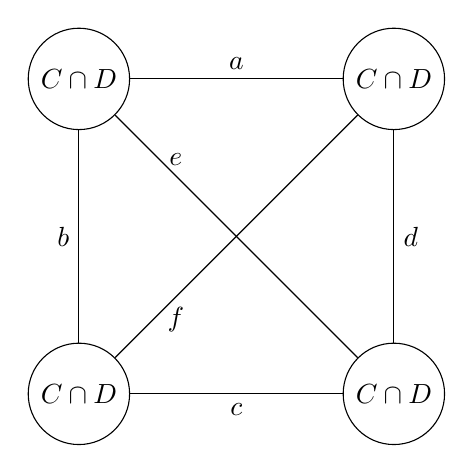
\begin{tikzpicture}
    \node[shape=circle,draw=black] (A) at (0,4) {\(C \cap D\)};
    \node[shape=circle,draw=black] (B) at (4,4) {\(\stcomp{C} \cap D\)};
    \node[shape=circle,draw=black] (C) at (4,0) {\(\stcomp{C} \cap \stcomp{D}\)};
    \node[shape=circle,draw=black] (D) at (0,0) {\(C \cap \stcomp{D}\)};
    
    \path (A) edge node [above] {\(a\)} (B);
    \path (A) edge node [near start, above] {\(e\)} (C);
    \path (A) edge node [left] {\(b\)} (D);
    \path (B) edge node [right] {\(d\)} (C);
    \path (B) edge node [near end, below] {\(f\)} (D);
    \path (C) edge node [below] {\(c\)} (D);
    \end{tikzpicture}
    \caption{The four cuts and their all possible edge boundaries between them. Diagram taken from \cite[p.~4]{Kr90}.}
    \label{fig:cuts}
    \end{figure}

    Let 
    \begin{align*}
        a &= |\partial(C \cap D, \stcomp{C} \cap D)|, & d &= |\partial(\stcomp{C} \cap D, \stcomp{C} \cap \stcomp{D})|, \\
        b &= |\partial(C \cap D, C \cap \stcomp{D})|, & e &= |\partial(C \cap D, \stcomp{C} \cap \stcomp{D})|, \\
        c &= |\partial(C \cap \stcomp{D}, \stcomp{C} \cap \stcomp{D})|, & f &= |\partial(C \cap \stcomp{D}, \stcomp{C} \cap D)|.
    \end{align*}

    Then, 

    \begin{align*}
    \kappa &= |\partial(C)| \\
           &= |\partial(C, \stcomp{C})| \\
           &= |\partial(C, \stcomp{C} \cap D)| + |\partial(C, \stcomp{C} \cap \stcomp{D})| \\
           &= |\partial(C \cap D, \stcomp{C} \cap D)| + |\partial(C \cap \stcomp{D}, \stcomp{C} \cap D)| \\
           &\quad + |\partial(C \cap D, \stcomp{C} \cap \stcomp{D})| + |\partial(C \cap \stcomp{D}, \stcomp{C} \cap \stcomp{D})| \\
           &= a + f + e + c. && \text{(1)} \\
    \intertext{This corresponds exactly to the edges in the diagram emanating from \(C \cap D\) and \(C \cap \stcomp{D}\). Similarly,}
    \kappa &= |\partial(D)| = b + f + e + d. && \text{(2)} 
    \intertext{By (1) and (2),}
        2\kappa &= a + b + c + d + 2e + 2f. && \text{(3)} 
    \intertext{The sets \(C \cap D\) and \(\stcomp{C} \cap \stcomp{D}\) contain an end, %go over this part
    so \(\partial(C \cap D) = a + e + b \geq \kappa\) and \(\partial(\stcomp{C} \cap \stcomp{D}) = c+e+d \geq \kappa\). It follows that the sum \(a+b+c+d+2e \geq 2\kappa\). By comparison with (3), we have that \(f = 0\). Finally,}
    \kappa &= a + e + b = c + e + d.
    \intertext{Therefore, \(\partial(C \cap D)\) and \(\partial(\stcomp{C} \cap \stcomp{D})\) are minimal as required.} \altqedhere
\end{align*} 
\end{proof}

\subsubsection{Building structure trees}
Our goal in this section is to shed light on how to construct \emph{structure trees}, as in \cite{K10} and \cite{D13}. In particular, we are interested in the action of finitely generated groups with more than one end on structure trees of their Cayley graphs, and how this ties in with our aim of proving Stallings' theorem. As the construction is very detailed, we focus instead on providing some intuition without going into detail about the proofs.

To start, note that if \(\Gamma\) is the Cayley graph of a group \(G\) with respect to some finite generating set \(S \subseteq G\), then \(\Gamma\) is connected and the action of \(G\) on \(\Gamma\) is transitive (there is only one orbit of vertices).

\begin{definition}[Nested]
    Cuts of vertices \(C, D \subset V(\Gamma)\) are \emph{nested} if one of the following conditions hold:
    \begin{enumerate}
        \item \(C \subset D\)
        \item \(D \subset C\)
        \item \(C \cap D = \varnothing\)
        \item \(C \cup D = V(\Gamma)\).
    \end{enumerate}
    Alternatively, cuts are nested if there is one empty corner. Cuts \(C,D\) are said to be \emph{non-nested} if they are not nested.
\end{definition}

Structure trees are trees which are constructed from \emph{structure cuts}, which are cuts \(C\) such that for any automorphism \(g \in \mathrm{Aut}(\Gamma)\), \(C\) and \(g(C)\) are nested. Let \(\mathcal{C} := \{g(C) \mid g \in \mathrm{Aut}(\Gamma)\}\) be this collection of cuts. If \(G\) acts on its Cayley graph \(\Gamma\), and if \(\mathcal{C}\) is a \(G\)-invariant set of nested cuts, then the action of \(G\) on \(\Gamma\) induces an action of \(G\) on a subset of the elements of \(\mathcal{C}\), which are called \(\mathcal{C}\)-blocks. From these \(\mathcal{C}\)-blocks, we can construct a tree --- in which \(\mathcal{C}\)-blocks form the vertices and edges are given by intersecting pairs of \(\mathcal{C}\)-blocks. The resulting tree is denoted \(T(\mathcal{C})\) and is called the \emph{structure tree}. If the action is transitive on \(\Gamma\), then it is also transitive on \(T(\mathcal{C})\).

Now that we have a transitive action on a infinite tree, Kr\"{o}n uses Bass-Serre theory to deduce that the group \(G\) splits over the stabiliser of an edge. As the action of a tree on its Cayley graph is free, there is some work to be done to show that the edge stabilisers of \(T(\mathcal{C})\) are finite.
In summary, this points to the following theorem:

\begin{theorem}[Opposite direction to Theorem~\ref{backimp}]
    Let \(G\) be an infinite finitely generated group with more than one end. Then, \(G\) splits over some finite subgroup \(H\). 
\end{theorem}

\begin{remark}
    There are many further details which have been omitted from the explanation above: for example, how do we define \(\mathcal{C}\)-blocks and how exactly does the action of \(G\) on its Cayley graph induce an action on these blocks? We will not address these in full, but instead will draw upon an example taken from \cite[p.~14]{D13}.
\end{remark}

\begin{figure}[h!]
    \centering
    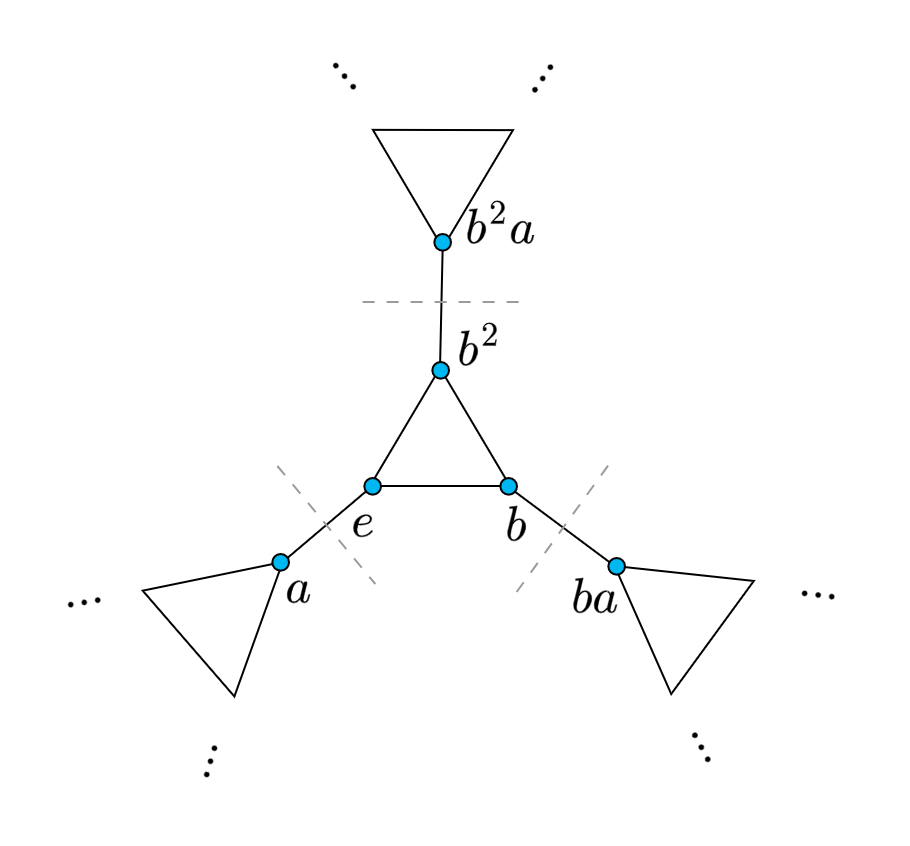
\includegraphics[width=0.6\linewidth]{sections/talia/CayleyGraph.png}
    \caption{A Cayley graph for \(\mathrm{PSL}(2,\mathbb{Z})\) with generating set \(\{a,b,a^{-1},b^{-1}\}\). The cuts are shown by dotted lines, and blue vertices form the block corresponding to this set of cuts.}
    \label{fig:psl}
\end{figure}

\begin{example}[Blocks in a Cayley graph for \(\mathrm{PSL}(2,\mathbb{Z})\)]
    
    Here, we use without proof that 
    \[
    \mathrm{PSL}(2,\mathbb{Z}) \cong \mathbb{Z}/2\mathbb{Z} * \mathbb{Z}/3\mathbb{Z} = \langle a,b \mid a^2 = b^3 =1 \rangle.
    \]
    Let the Cayley graph of \(\mathrm{PSL}(2,\mathbb{Z})\) generated by \(a, b\) and their inverses be called \(\Gamma\).
    Consider the three cuts denoted by the dotted lines in Figure~\ref{fig:psl}. The vertices in each cut lie in each of the three connected components which extend outwards toward infinity from each of the three dotted lines respectively. These three cuts form a set \(\mathcal{C}\), and the block relative to this \(\mathcal{C}\) is given by the blue vertices.
\end{example}

\begin{comment}
\subsubsection{Nested cuts}
\textcolor{cyan}{I don't really like this section. I feel like I can follow the individual theorems but I don't really understand what this part of the paper is trying to say. I'm going to try to replace this.}
Our goal in this section is to briefly explore how to construct \emph{structure trees}. In particular, we are interested in the action of finitely generated groups with more than one end on structure trees of their Cayley graphs. In order to build these trees, we introduce what is means for cuts to be \emph{nested}. Several results in this section are stated without proof, however proofs can be found in \cite[Chapter~3]{K10}. 

Recall the four cuts \(C \cap D, \stcomp{C} \cap D, C \cap \stcomp{D}, \stcomp{C} \cap \stcomp{D}\) which we referred to as \emph{corners} of \(C\) and \(D\). We say that the cuts which lie on diagonal corners of the diagram in Figure~\ref{fig:cuts} are \emph{opposite}.

\begin{definition}[Nested]
    Cuts of vertices \(C, D \subset V(\Gamma)\) are \emph{nested} if one of the following conditions hold:
    \begin{enumerate}
        \item \(C \subset D\)
        \item \(D \subset C\)
        \item \(C \cap D = \varnothing\)
        \item \(C \cup D = V(\Gamma)\).
    \end{enumerate}
    Alternatively, cuts are nested if there is one empty corner. Cuts \(C,D\) are said to be \emph{non-nested} if they are not nested.
\end{definition}

\begin{lemma}
    Let \(C, D, E\) be cuts of vertices and let \(C\) and \(D\) be non-nested. 
    \begin{enumerate}[(i)]
    \item If \(E\) is non-nested with two opposite corners of \(C\) and \(D\), then \(E\) is non-nested with both \(C\) and \(D\). 
    \item If \(E\) is non-nested with some corner of \(C\) and \(D\), then \(E\) is either non-nested with \(C\) or non-nested with \(D\).
    \end{enumerate}
\end{lemma}

\begin{remark}
  Note that this theorem does not hold when \(C,D,E\) are arbitrary sets of vertices instead of cuts.  
\end{remark}

\begin{example}
    Let \(\Gamma\) be the Cayley graph of \(F_2\) with generating set \(\{a,b,a^{-1},b^{-1}\}\). Let \(C\) be the ray given by \(\{e,a,a^2,a^3, \dots\}\), \(D = \{e, b, b^2, b^3 \dots\}\) and \(E = \{e, a, ab, aba,  \dots\}\). The sets \(C, D\) are non-nested. The corners of \(C\) and \(D\) are the following.
    \begin{align*}
        C \cap D & = \{e\} \\
        \stcomp{C} \cap D & = \{b,b^2,b^3,\dots\} \\
        C \cap \stcomp{D} & = \{a,a^2,a^3, \dots\} \\
        \stcomp{C} \cap \stcomp{D} & = \langle a,b \rangle \setminus \left\{ \langle a \rangle \cup \langle b \rangle \right\}
    \end{align*}
    The vertex set \(E\) is non-nested with the first corner, but non-nested with the others. By (i), we expect that \(E\) is non-nested with \(C\) and with \(D\), and one can verify that this is the case.
\end{example}

\begin{definition}[Minimal non-nested cuts]
    Let \(C\) be a cut and let \(M(C)\) be the set of minimal cuts which are non-nested with \(C\). Let \(m(C) = |M(C)|\) be the cardinality of this set. 
\end{definition}

\begin{lemma}
\label{lem:ineq}
    Let \(C\) and \(D\) be non-nested cuts and suppose \(C \cap D\) and \(\stcomp{C} \cap \stcomp{D}\) are cuts. Then,
    \[
        m(C \cap D) + m(\stcomp{C} \cap \stcomp{D}) < m(C) + m(D).
    \]
\end{lemma}

\begin{definition}
    Let \(\mathcal{C}\) be the set of all minimal cuts. Set \(m = \min\{m(C) \mid C \in \mathcal{C}\}\).  A minimal cut \(C\) with \(m(C) = m\) is called \emph{optimally nested}.
\end{definition}

\begin{theorem}
    Optimally nested cuts are nested with all other optimally nested cuts.
\end{theorem}

\begin{proof}
    \cite[Theorem~3.3, p.~5--6]{K10}
    Suppose there are optimally nested minimal cuts \(E\) and \(F\) which are non-nested. Then \(m \geq 1\). There cannot be two adjacent corners which do not contain an end, because \(C, D, \stcomp{C}\) and \(\stcomp{D}\) all contain an end (since they are cuts and must contain a ray by definition, and contain all equivalent rays by Proposition~\ref{prop:ray}). Hence there is a pair of opposite corners which contain an end. By relabeling, we can assume that these corners are \(C \cup D\) and \(\stcomp{C} \cap \stcomp{D}\) and by Lemma~\ref{lem:mincuts}, \(C \cap D\) and \(\stcomp{C} \cap \stcomp{D}\) are minimal cuts.
    Using Lemma~\ref{lem:ineq},
    \[
    m(C \cap D) + m(\stcomp{C} \cap \stcomp{D}) < m(C) + m(D) = 2m.
    \]
    Therefore, one of the summands on the left side is less than \(m\), contradicting the minimality of \(m\). 
\end{proof}

\textcolor{cyan}{Once I understand this I really want to reinforce why this theorem is important and why we care about nested cuts. Kron talks about G-invariant automorphisms and this feels important}

From these systems of nested cuts, one can build a tree known as the \emph{structure tree}. 

With a few more definitions, we conclude this section by illustrating this construction.

\begin{definition}[Boundary of a cut]
    Let \(C\) be a cut. The \emph{boundary} of \(C\), denoted by \(\Delta(C)\), is the set of vertices in \(\stcomp{C}\) which are adjacent to a vertex in \(C\).
\end{definition}

\begin{definition}[Blocks]
    Let \(\mathcal{C}\) be a set of cuts. A maximal set of vertices \(B\) for which the following condition is satisfied is called a \(\mathcal{C}\)-block. 
    The condition is as follows: for all \(C \in \mathcal{C}\), either \(B \subset C \cup \Delta(C)\) or \(B \subset \stcomp{C} \cup \stcomp{\Delta(C)}\).
\end{definition}

\begin{definition}[Nested set of cuts]
    A set of minimal cuts \(\mathcal{C}\) is \emph{nested} if any two cuts \(C, D \in \mathcal{C}\) are nested. 
\end{definition}

\begin{construction}[Structure tree]
\label{const:structuretree}
    Given a nested set \(\mathcal{C}\) of minimal cuts, we define a graph \(T = T(\mathcal{C})\).
    \begin{itemize}
        \item Take the vertex set \(V(T)\) to be the set of \(\mathcal{C}\)-blocks.
        \item Two vertices are adjacent if they intersect as \(\mathcal{C}\)-blocks.
    \end{itemize}
\end{construction}

\begin{lemma}
\cite[Theorem~4.2,p.~7]{K10}
    The structure tree defined in Construction~\ref{const:structuretree} is a tree.
\end{lemma}
\end{comment}

\subsection{Links to Bass--Serre theory and further questions}
\subsubsection{Generalisations}
Stallings' structure theorem in the language of Bass--Serre theory gives the following useful corollary. 
\begin{corollary}
    A finitely generated group with more than one end has a non-trivial action on a tree with finite edge stabilisers.
\end{corollary}

Furthermore, from Stallings' structure theorem we can derive an even stronger classification.
\begin{theorem}[Stalling's Structure Theorem II]
    Stallings' structure theorem (Theorem~\ref{thm:SST}) extends to the following classification: 
    \begin{itemize}
        \item (1) corresponds to the case in which \(G\) has exactly two ends,
        \item (2) corresponds to the case where \(G\) has infinitely many ends and is torsion-free, and
        \item (3) corresponds to the case where \(G\) has infinitely many ends and has torsion.
    \end{itemize}
\end{theorem}

It seems that there is no similar classification for one-ended groups. Since most finitely generated infinite groups are not virtually \(\mathbb{Z}\) and cannot be split over a finite subgroup, we can take away the conclusion that most infinite finitely generated groups are in fact one-ended.

\subsubsection{Further research}
There is plenty more to be explored here and we give two possible directions for further investigation. 

\textbf{1.} \textit{``If most finitely generated groups are one-ended, what are some other examples other than \(\mathbb{Z}^2\)?''} 

In particular, a large class of hyperbolic groups are one-ended:

\begin{theorem} \cite{S96}
    A hyperbolic group is one-ended if its Gromov boundary is a non-empty connected space.
\end{theorem}

Hence, a set of examples would be the surface groups \(\pi_1(\Sigma_g)\) for \(g \geq 2\). One could look into similar theorems for small cancellation, Fuschian, or right-angled Artin groups.

\vspace{1em}
\textbf{2.} \textit{``Does there exist a notion of ends of a group for an infinitely generated group? Do Stallings' results generalise further in this direction?''}
The answer to both of these questions is yes. The definition of such an end and the theorem below is given in \cite{phdthesis} (originally \cite{D89}).

\begin{theorem}
     Let \(G\) be a group. The following are equivalent:
     \begin{enumerate}[(i)]
         \item \(e(G) > 1\).
         \item For any non-trivial free \(G\)-module \(M\), \(H^1(G,M) \neq 0\).
         \item There exists a tree on which \(G\) acts without global fixed points and finite edge stabilisers.
         \item One of the following holds:
         \begin{itemize}
             \item \(G\) splits as an amalgam over a finite subgroup \(H\),
             \item \(G\) splits as a HNN-extension over a finite subgroup \(H\),
             \item \(G\) is countably infinite and locally finite.
         \end{itemize}
         \item \(e(G) = 2\) or \(e(G) = \infty\).
     \end{enumerate}
\end{theorem}
